\section{Introduction}

Manipulation of deformable objects is an area of robotics research that has received attention from several diverse fields in recent years. Examples of deformable object manipulation range from domestic tasks like folding clothes to time and safety critical tasks such as robotic surgery. One of the primary challenges in manipulating deformable objects is the difficulty of modeling and simulating them. Motivated by applications in computer graphics and surgical training, many methods have been developed for simulating string-like objects \cite{Bergou2008,Rungjiratananon2011}, cloth-like objects \cite{Baraff1998,Goldenthal2007}, and tissue-like objects \cite{Sutherland2006,Chentanez2009,Kim2007}. The most common simulation methods use Mass-Spring models \cite{Gibson1997,Essahbi2012}, which are generally not accurate for large deformations \cite{Maris2010}, and Finite-Element models \cite{Muller2002,Irving2004,Bathe2006}, which require significant tuning and are very sensitive to the discretization of the object. Approaches like \cite{Schulman2016,Huang2015} bypass this challenge by using offline demonstrations to teach the robot specific manipulation tasks; however, when a new task is attempted a new training set needs to be generated. In our application we are interested in a way to manipulate a deformable object without a high-fidelity model or training set available \textit{a priori}. For instance, imagine a robot encountering a new piece of clothing for a new task. While it may have models for previously-seen clothes or training sets for previous tasks, there is no guarantee that those models or training sets are appropriate for the new task. Also, depending on the state of the clothing different models may be most useful at different times in the manipulation task.

\begin{figure}[t]
    \centering
    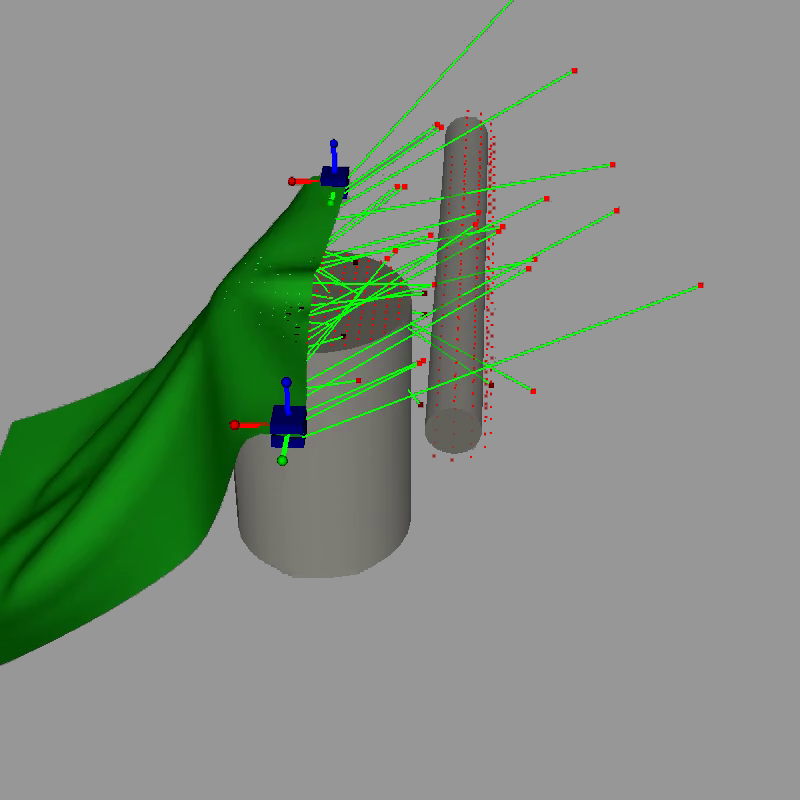
\includegraphics[width=\columnwidth,trim={1cm 7cm 3cm 3cm},clip]{cloth_wafr_intro_image}
    \caption{An example manipulation task in simulation.}
    \label{fig:intro_figure}
\end{figure}

Rather than assuming we have a high-fidelity model of a deformable object interacting with its environment, our approach is to have multiple models available for use, any one of which may be useful at a given time. We do not assume these models are correct, we simply treat the models as having some measurable \textit{utility} to the task. The \textit{utility} of a given model is the expected reduction in task error when using this model to generate robot motion. As the task proceeds, the utility of a given model may change, making other models more suitable for the current part of the task. However, without testing a model's prediction, we do not know its true utility. Testing every model in the set is impractical, as all models would need to be tested at every step, and performing a test changes the state of the object and may drive it into a local minimum. The key question is then which model should be selected for testing at a given time.

The central contribution of this paper is framing the model selection problem as a Multi-Armed Bandit (MAB) problem where the goal is to find the model that has the highest utility for a given task. An arm represents a single model of the deformable object; to ``pull'' an arm is to use the arm's model to generate and execute a velocity command for the robot. The reward received is the reduction in task error after executing the command. In order to determine which model has the highest utility we need to explore the model space, however we also want to exploit the information we have gained by using models that we estimate to have high utility. One of the primary challenges in performing this exploration versus exploitation trade-off is that our models are inherently coupled and non-stationary; performing an action changes the state of the system which can change the utility of every model, as well as the reward of pulling each arm. While there is work that frames robust trajectory selection as a MAB problem~\cite{Koval2015}, we are not aware of any previous work which either 1) frames model selection for deformable objects as a MAB problem; or 2) addresses the coupling between arms for non-stationary MAB problems.

In our experiments, we show how to formulate a MAB problem with coupled arms for Jacobian-based models. We perform our experiments on three synthetic systems, and on three deformable object manipulation tasks in the Bullet Physics~\cite{Coumans2010} simulator (Fig.~\ref{fig:intro_figure}). We demonstrate that formulating model selection as a MAB problem is able to successfully perform all three manipulation tasks. We also show that our proposed MAB algorithm outperforms previous MAB methods on synthetic trials, and performs competitively on the manipulation tasks.

This paper is an extension of our previous work~\cite{dale_wafr}. We have included additional related work, more details of the algorithms, as well as additional discussion.